\documentclass[tikz,border=10pt]{standalone}
\begin{document}
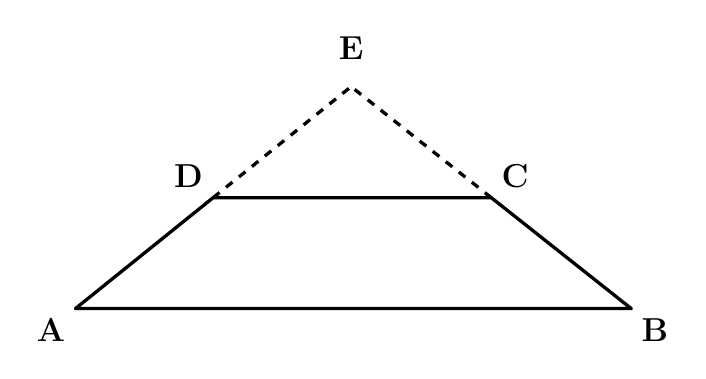
\begin{tikzpicture}[line width=0.8pt, line join=round]
  % Vertices (scale s = 0.014981 cm per px, origin near figure centre)
  \coordinate (A) at (-3.528,-1.408);
  \coordinate (B) at (3.531,-1.408);
  \coordinate (C) at (1.754,0);
  \coordinate (D) at (-1.780,0);
  \coordinate (E) at (-0.027,1.411);

  % Solid trapezoid edges AB, BC, CD, DA (heavier stroke)
  \draw[line width=1.2pt] (A) -- (B) -- (C) -- (D) -- cycle;

  % Dashed extensions of legs to apex E (heavier stroke, dashed kept)
  \draw[dashed, line width=1.2pt] (D) -- (E);
  \draw[dashed, line width=1.2pt] (C) -- (E);

  % Bold labels; E shifted further above its apex
  \node[font=\fontsize{12}{14.4}\selectfont, below left] at (A) {$\mathbf{A}$};
  \node[font=\fontsize{12}{14.4}\selectfont, below right] at (B) {$\mathbf{B}$};
  \node[font=\fontsize{12}{14.4}\selectfont, above right] at (C) {$\mathbf{C}$};
  \node[font=\fontsize{12}{14.4}\selectfont, above left] at (D) {$\mathbf{D}$};
  \node[font=\fontsize{12}{14.4}\selectfont, above=6pt] at (E) {$\mathbf{E}$};
\end{tikzpicture}
\end{document}